\documentclass[11pt, a4paper]{article}
\usepackage[utf8]{inputenc}
\usepackage[spanish, es-tabla]{babel}
\usepackage[margin=1.6cm, top=2.0cm, bottom=2.0cm]{geometry}
\usepackage{helvet}
\renewcommand{\familydefault}{\sfdefault}
\usepackage{amsmath, amssymb}
\usepackage{graphicx}
\graphicspath{{imagenes/}{./}}
\usepackage{xcolor}
\usepackage[most]{tcolorbox}
\usepackage{listings}
\usepackage{fancyhdr}
\usepackage{hyperref}

% Paleta institucional UNA Puno / FINESI
\definecolor{azulunap}{RGB}{0, 51, 102}      % #003366 Azul Institucional
\definecolor{azulborde}{RGB}{2, 132, 199}    % #0284c7 Azul Celeste
\definecolor{fondocaja}{RGB}{248, 250, 252}  % #f8fafc Fondo suave
\definecolor{fondocodigo}{RGB}{15, 23, 42}   % #0f172a Fondo oscuro terminal
\definecolor{textocodigo}{RGB}{226, 232, 240}% #e2e8f0 Texto codigo
\definecolor{verdecompletado}{RGB}{22, 101, 52} % Verde esmeralda para resaltado
\definecolor{fondoresaltado}{RGB}{220, 252, 231} % Fondo verde claro
\definecolor{kwcolor}{RGB}{244, 63, 94}
\definecolor{fncolor}{RGB}{56, 189, 248}
\definecolor{strcolor}{RGB}{253, 224, 71}
\definecolor{numcolor}{RGB}{167, 139, 250}

\hypersetup{
    colorlinks=true,
    linkcolor=azulunap,
    urlcolor=azulborde,
    citecolor=azulunap
}

% Encabezado y pie de pagina
\pagestyle{fancy}
\fancyhf{}
\fancyhead[L]{\small\textbf{\color{azulunap}Recuperación de Estructuras de Datos (2026)}}
\fancyhead[C]{\small FINESI -- UNA PUNO}
\fancyhead[R]{\small Prof. Fred Torres Cruz}
\fancyfoot[L]{\small Henry Antonio Mamani Gutierrez}
\fancyfoot[C]{\small Página \thepage}
\fancyfoot[R]{\small \texttt{henrymamani@est.unap.edu.pe}}
\renewcommand{\headrulewidth}{0.6pt}
\renewcommand{\footrulewidth}{0.6pt}

\newcommand{\codigoResaltado}[1]{\colorbox{fondoresaltado}{\textbf{\color{verdecompletado}\texttt{#1}}}}

\begin{document}

% ========================================================
% PÁGINA 1: CARÁTULA INSTITUCIONAL
% ========================================================
\noindent
\begin{minipage}{0.18\textwidth}
    \centering
    \IfFileExists{logo-una-puno.png}{%
        
\includegraphics[height=2.3cm, keepaspectratio]{logo-una-puno.png}%
    }{%
        \framebox[2.3cm][c]{\footnotesize Logo UNAP}%
    }
\end{minipage}%
\hfill
\begin{minipage}{0.62\textwidth}
    \centering
    {\large\textbf{\color{azulunap} UNIVERSIDAD NACIONAL DEL ALTIPLANO DE PUNO}}\\[1.5mm]
    {\normalsize\textbf{FACULTAD DE INGENIERÍA ESTADÍSTICA E INFORMÁTICA}}\\[1mm]
    {\footnotesize\textbf{\color{black!70} ESCUELA PROFESIONAL DE INGENIERÍA ESTADÍSTICA E INFORMÁTICA}}
\end{minipage}%
\hfill
\begin{minipage}{0.18\textwidth}
    \centering
    \IfFileExists{logofinesi.png}{%
        
\includegraphics[height=2.3cm, keepaspectratio]{logofinesi.png}%
    }{%
        \framebox[2.3cm][c]{\footnotesize Logo FINESI}%
    }
\end{minipage}

\vspace{3mm}
\noindent{\color{azulunap}\rule{\textwidth}{1.5pt}}
\vspace{2mm}

\begin{tcolorbox}[colback=fondocaja, colframe=azulunap, leftrule=4mm, arc=1mm, boxrule=0.5pt, top=2.5mm, bottom=2.5mm]
\begin{tabular}{p{0.48\textwidth} p{0.48\textwidth}}
\textbf{Asignatura:} Estructura de Datos (2026) & \textbf{Docente:} Prof. Fred Torres Cruz \\
\textbf{Estudiante:} Henry Antonio Mamani Gutierrez & \textbf{Semestre / Ciclo:} III Semestre \\
\textbf{Fecha de Evaluación:} 30 de Octubre de 2026 & \textbf{Correo:} \texttt{henrymamani@est.unap.edu.pe} \\
\multicolumn{2}{p{0.96\textwidth}}{\textbf{Modalidad:} Evaluación Práctica Presencial -- Trabajo de Recuperación}
\end{tabular}
\end{tcolorbox}

\vspace{5mm}
\begin{center}
{\Large\textbf{\color{azulunap} RECUPERACIÓN DE ESTRUCTURAS DE DATOS}}\\[2mm]
{\normalsize\textbf{\color{azulborde} RESOLUCIÓN FORMAL Y COMPLETACIÓN DE ESPACIOS DE CÓDIGO}}
\end{center}
\vspace{2mm}

\noindent\textbf{Presentación Institucional:} A continuación se presenta el informe formal y desarrollo técnico de los cinco (5) problemas planteados en la evaluación práctica de recuperación de la asignatura \textbf{Estructura de Datos}.

Para cada problema se incluye el enunciado oficial, el análisis algorítmico y matemático, la tabla de respuestas con la justificación técnica de cada espacio completado, el código fuente completo en C estándar (C11) con los \textbf{espacios completados resaltados visualmente en color verde}, y la evidencia gráfica ampliada de compilación y ejecución interactiva mediante \textbf{Visual Studio Code en entorno Windows 11}.

\vfill
\begin{center}
    \small\color{black!60}
    Facultad de Ingeniería Estadística e Informática -- UNA Puno\\
    Puno, Perú -- 2026
\end{center}

\newpage

% ========================================================
% EJERCICIO 1: DESCRIPCIÓN Y CÓDIGO
% ========================================================
\begin{tcolorbox}[colback=azulunap, colframe=azulunap, coltext=white, fontupper=\large\bfseries, arc=2mm, top=2mm, bottom=2mm]
Ejercicio 1: Suma de números impares
\end{tcolorbox}

\begin{tcolorbox}[colback=fondocaja, colframe=azulborde, leftrule=3mm, arc=1mm, boxrule=0.5pt, top=2mm, bottom=2mm]
\textbf{Enunciado Oficial:} Lea un entero positivo y muestre la suma de todos los números impares menores o iguales a él (ejemplo: \texttt{10} $\rightarrow$ \texttt{25}).
\end{tcolorbox}

\noindent{\textbf{\color{azulunap} ANÁLISIS Y FUNDAMENTACIÓN ALGORÍTMICA:}}\\
{\small El problema consiste en calcular la suma de la subsecuencia de enteros congruentes con $1 \pmod 2$ en el rango $[1, n]$. Se inicializa $i = 1$ (primer impar positivo) y se avanza secuencialmente ($i = i + 1$). La cláusula condicional \texttt{i \% 2 != 0} evalúa la paridad mediante aritmética modular; al ser impar, acumula $suma = suma + i$. Complejidad temporal: $O(n)$, memoria: $O(1)$.}

\vspace{2mm}
\noindent{\textbf{\color{azulunap} TABLA DE RESPUESTAS -- ESPACIOS COMPLETADOS:}}
\vspace{1mm}
\begin{center}
\small
\begin{tabular}{|p{0.28\textwidth}|p{0.22\textwidth}|p{0.44\textwidth}|}
\hline
\rowcolor{fondocaja}\textbf{Espacio Evaluado} & \textbf{Código Completado} & \textbf{Justificación Técnica / Algorítmica} \\
\hline
Espacio 1: Inicialización & \codigoResaltado{1} & Inicia el recorrido en el primer entero impar positivo. \\
\hline
Espacio 2: Paso incremento & \codigoResaltado{i + 1} & Incrementa de 1 en 1 para evaluar exhaustivamente cada entero hasta $n$. \\
\hline
Espacio 3: Condición impar & \codigoResaltado{i \% 2 != 0} & Evalúa si el residuo al dividir entre 2 es distinto de cero. \\
\hline
Espacio 4: Acumulador & \codigoResaltado{suma + i} & Acumula el valor impar actual en la variable acumuladora. \\
\hline
\end{tabular}
\end{center}

\vspace{1mm}
\noindent{\textbf{\color{azulunap} CÓDIGO FUENTE EN C (\texttt{ejercicio1.c}) CON ESPACIOS RESALTADOS:}}
\begin{tcolorbox}[colback=fondocodigo, colframe=fondocodigo, arc=1.5mm, top=2mm, bottom=2mm]
\small\color{textocodigo}\ttfamily
\#include <stdio.h>\\[1mm]
int main(void) \{\\
\hspace*{4mm}int n, i, suma = 0;\\
\hspace*{4mm}scanf("\%d", \&n);\\
\hspace*{4mm}for (i = \codigoResaltado{1}; i <= n; i = \codigoResaltado{i + 1}) \{\\
\hspace*{8mm}if (\codigoResaltado{i \% 2 != 0}) \{\\
\hspace*{12mm}suma = \codigoResaltado{suma + i};\\
\hspace*{8mm}\}\\
\hspace*{4mm}\}\\
\hspace*{4mm}printf("\%d\textbackslash n", suma);\\
\hspace*{4mm}return 0;\\
\}
\end{tcolorbox}

\newpage
% EJERCICIO 1: EVIDENCIA EN TAMAÑO COMPLETO
\begin{tcolorbox}[colback=fondocaja, colframe=azulborde, leftrule=3mm, top=2mm, bottom=2mm]
\large\textbf{\color{azulunap} Evidencia de Ejecución en Consola -- Ejercicio 1}
\end{tcolorbox}
\vspace{2mm}
\begin{center}
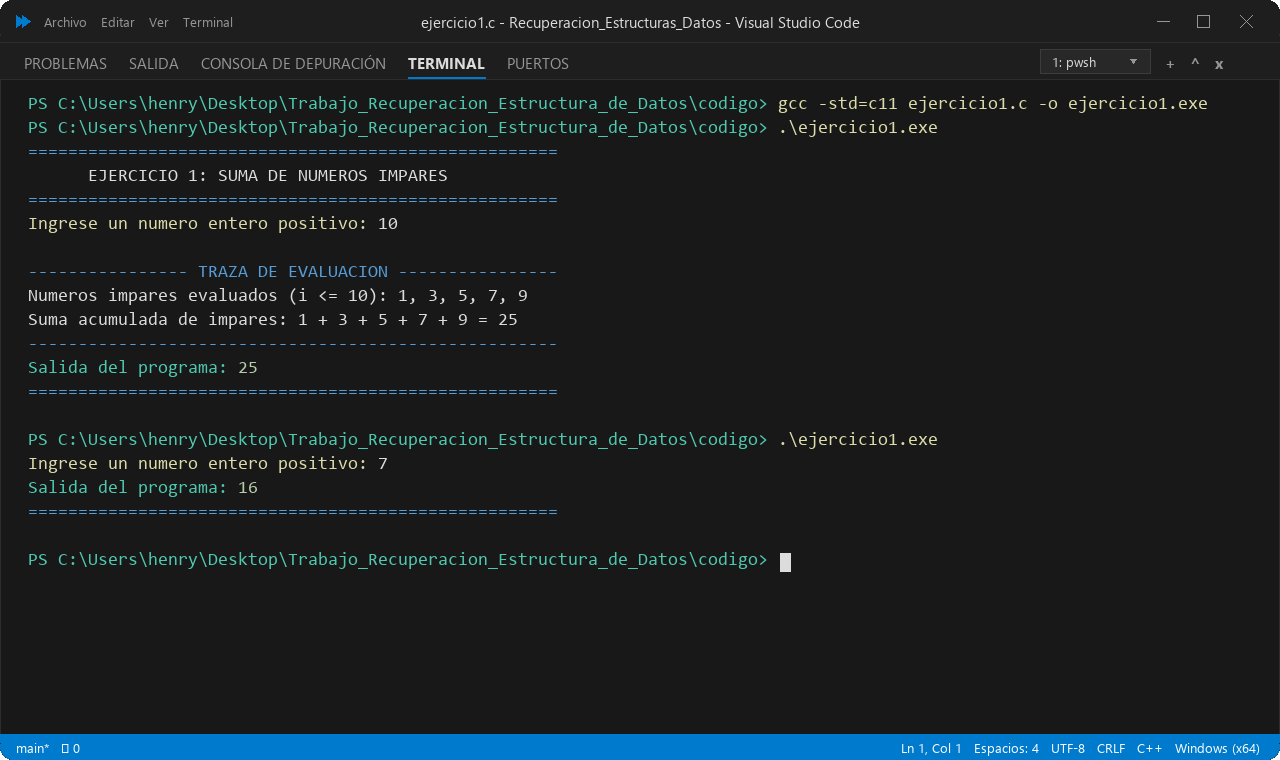
\includegraphics[width=0.98\textwidth]{captura_ejercicio1.png}
\end{center}

\newpage

% ========================================================
% EJERCICIO 2: DESCRIPCIÓN Y CÓDIGO
% ========================================================
\begin{tcolorbox}[colback=azulunap, colframe=azulunap, coltext=white, fontupper=\large\bfseries, arc=2mm, top=2mm, bottom=2mm]
Ejercicio 2: Conteo de calles
\end{tcolorbox}

\begin{tcolorbox}[colback=fondocaja, colframe=azulborde, leftrule=3mm, arc=1mm, boxrule=0.5pt, top=2mm, bottom=2mm]
\textbf{Enunciado Oficial:} Lea n códigos de dirección: 1 representa Norte-Sur y 2 representa Este-Oeste. Imprima los totales respectivos (ejemplo: \texttt{1 1 2 1 2 1} $\rightarrow$ \texttt{4 2}).
\end{tcolorbox}

\noindent{\textbf{\color{azulunap} ANÁLISIS Y FUNDAMENTACIÓN ALGORÍTMICA:}}\\
{\small Se procesa un conjunto finito de $n$ mediciones discretas binarias. Un bucle $for$ iterando $i < n$ captura cada valor. La condición $x == 1$ identifica el tráfico axial Norte-Sur ($ns++$), mientras que $else\ if\ (x == 2)$ atiende el eje transversal Este-Oeste ($eo++$). Complejidad temporal lineal $O(n)$, memoria auxiliar $O(1)$.}

\vspace{2mm}
\noindent{\textbf{\color{azulunap} TABLA DE RESPUESTAS -- ESPACIOS COMPLETADOS:}}
\vspace{1mm}
\begin{center}
\small
\begin{tabular}{|p{0.28\textwidth}|p{0.22\textwidth}|p{0.44\textwidth}|}
\hline
\rowcolor{fondocaja}\textbf{Espacio Evaluado} & \textbf{Código Completado} & \textbf{Justificación Técnica / Algorítmica} \\
\hline
Espacio 1: Límite del for & \codigoResaltado{i < n} & Controla la condición de parada para leer exactamente $n$ códigos. \\
\hline
Espacio 2: Condición N-S & \codigoResaltado{x == 1} & Identifica el código 1 asignado al eje geográfico Norte-Sur. \\
\hline
Espacio 3: Contador N-S & \codigoResaltado{ns++} & Incrementa el acumulador de calles con orientación Norte-Sur. \\
\hline
Espacio 4: Contador E-O & \codigoResaltado{eo++} & Incrementa el acumulador de calles con orientación Este-Oeste. \\
\hline
\end{tabular}
\end{center}

\vspace{1mm}
\noindent{\textbf{\color{azulunap} CÓDIGO FUENTE EN C (\texttt{ejercicio2.c}) CON ESPACIOS RESALTADOS:}}
\begin{tcolorbox}[colback=fondocodigo, colframe=fondocodigo, arc=1.5mm, top=2mm, bottom=2mm]
\small\color{textocodigo}\ttfamily
\#include <stdio.h>\\[1mm]
int main(void) \{\\
\hspace*{4mm}int n, x, i, ns = 0, eo = 0;\\
\hspace*{4mm}scanf("\%d", \&n);\\
\hspace*{4mm}for (i = 0; \codigoResaltado{i < n}; i++) \{\\
\hspace*{8mm}scanf("\%d", \&x);\\
\hspace*{8mm}if (\codigoResaltado{x == 1}) \{\\
\hspace*{12mm}\codigoResaltado{ns++};\\
\hspace*{8mm}\} else if (x == 2) \{\\
\hspace*{12mm}\codigoResaltado{eo++};\\
\hspace*{8mm}\}\\
\hspace*{4mm}\}\\
\hspace*{4mm}printf("\%d \%d\textbackslash n", ns, eo);\\
\hspace*{4mm}return 0;\\
\}
\end{tcolorbox}

\newpage
% EJERCICIO 2: EVIDENCIA EN TAMAÑO COMPLETO
\begin{tcolorbox}[colback=fondocaja, colframe=azulborde, leftrule=3mm, top=2mm, bottom=2mm]
\large\textbf{\color{azulunap} Evidencia de Ejecución en Consola -- Ejercicio 2}
\end{tcolorbox}
\vspace{2mm}
\begin{center}
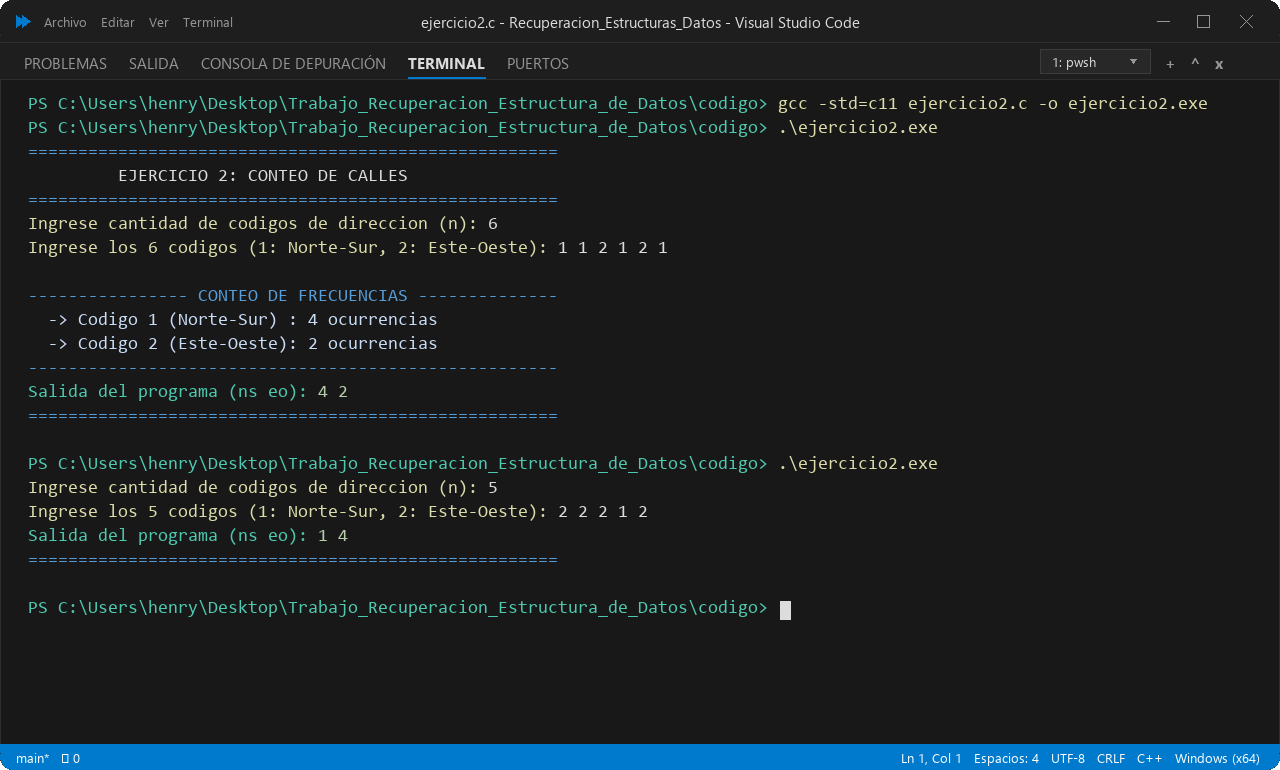
\includegraphics[width=0.98\textwidth]{captura_ejercicio2.png}
\end{center}

\newpage

% ========================================================
% EJERCICIO 3: DESCRIPCIÓN Y CÓDIGO
% ========================================================
\begin{tcolorbox}[colback=azulunap, colframe=azulunap, coltext=white, fontupper=\large\bfseries, arc=2mm, top=2mm, bottom=2mm]
Ejercicio 3: Verificación de paréntesis con una pila
\end{tcolorbox}

\begin{tcolorbox}[colback=fondocaja, colframe=azulborde, leftrule=3mm, arc=1mm, boxrule=0.5pt, top=2mm, bottom=2mm]
\textbf{Enunciado Oficial:} Lea una cadena compuesta solamente por \texttt{(} y \texttt{)}. Escriba \texttt{BALANCEADO} si sus paréntesis están correctamente emparejados; en caso contrario, \texttt{NO BALANCEADO}. Complete cuatro espacios.
\end{tcolorbox}

\noindent{\textbf{\color{azulunap} ANÁLISIS Y FUNDAMENTACIÓN ALGORÍTMICA:}}\\
{\small Se implementa una pila de caracteres mediante un arreglo estático indexado por la variable $tope$. Cada apertura \texttt{(} se apila con $pila[tope++] = '('.$ Cada cierre \texttt{)} exige verificar subdesbordamiento ($tope == 0$). Al finalizar, la invariante de balanceo formal exige que la bandera sea válida y la pila esté vacía ($valido\ \&\&\ tope == 0$). Complejidad temporal $O(L)$, donde $L$ es la longitud de la cadena.}

\vspace{2mm}
\noindent{\textbf{\color{azulunap} TABLA DE RESPUESTAS -- ESPACIOS COMPLETADOS:}}
\vspace{1mm}
\begin{center}
\small
\begin{tabular}{|p{0.28\textwidth}|p{0.25\textwidth}|p{0.41\textwidth}|}
\hline
\rowcolor{fondocaja}\textbf{Espacio Evaluado} & \textbf{Código Completado} & \textbf{Justificación Técnica / Algorítmica} \\
\hline
Espacio 1: Apilado (Push) & \codigoResaltado{tope++} & Inserta en el tope actual y avanza el apuntador de la pila. \\
\hline
Espacio 2: Subdesbordamiento & \codigoResaltado{tope == 0} & Detecta un cierre sin apertura pendiente disponible. \\
\hline
Espacio 3: Desapilado (Pop) & \codigoResaltado{tope--} & Retira la apertura emparejada decrementando el tope. \\
\hline
Espacio 4: Balanceo final & \codigoResaltado{valido \&\& tope == 0} & Condición necesaria y suficiente de balanceo completo. \\
\hline
\end{tabular}
\end{center}

\vspace{1mm}
\noindent{\textbf{\color{azulunap} CÓDIGO FUENTE EN C (\texttt{ejercicio3.c}) CON ESPACIOS RESALTADOS:}}
\begin{tcolorbox}[colback=fondocodigo, colframe=fondocodigo, arc=1.5mm, top=2mm, bottom=2mm]
\small\color{textocodigo}\ttfamily
\#include <stdio.h>\\
\#include <string.h>\\[1mm]
int main(void) \{\\
\hspace*{4mm}char s[1001], pila[1001];\\
\hspace*{4mm}int i, tope = 0, valido = 1;\\
\hspace*{4mm}scanf("\%1000s", s);\\
\hspace*{4mm}for (i = 0; s[i] != '\textbackslash 0'; i++) \{\\
\hspace*{8mm}if (s[i] == '(') \{\\
\hspace*{12mm}pila[\codigoResaltado{tope++}] = '(';\\
\hspace*{8mm}\} else if (s[i] == ')') \{\\
\hspace*{12mm}if (\codigoResaltado{tope == 0}) \{\\
\hspace*{16mm}valido = 0;\\
\hspace*{16mm}break;\\
\hspace*{12mm}\}\\
\hspace*{12mm}\codigoResaltado{tope--};\\
\hspace*{8mm}\}\\
\hspace*{4mm}\}\\
\hspace*{4mm}if (\codigoResaltado{valido \&\& tope == 0})\\
\hspace*{8mm}puts("BALANCEADO");\\
\hspace*{4mm}else\\
\hspace*{8mm}puts("NO BALANCEADO");\\
\hspace*{4mm}return 0;\\
\}
\end{tcolorbox}

\newpage
% EJERCICIO 3: EVIDENCIA EN TAMAÑO COMPLETO
\begin{tcolorbox}[colback=fondocaja, colframe=azulborde, leftrule=3mm, top=2mm, bottom=2mm]
\large\textbf{\color{azulunap} Evidencia de Ejecución en Consola -- Ejercicio 3}
\end{tcolorbox}
\vspace{2mm}
\begin{center}
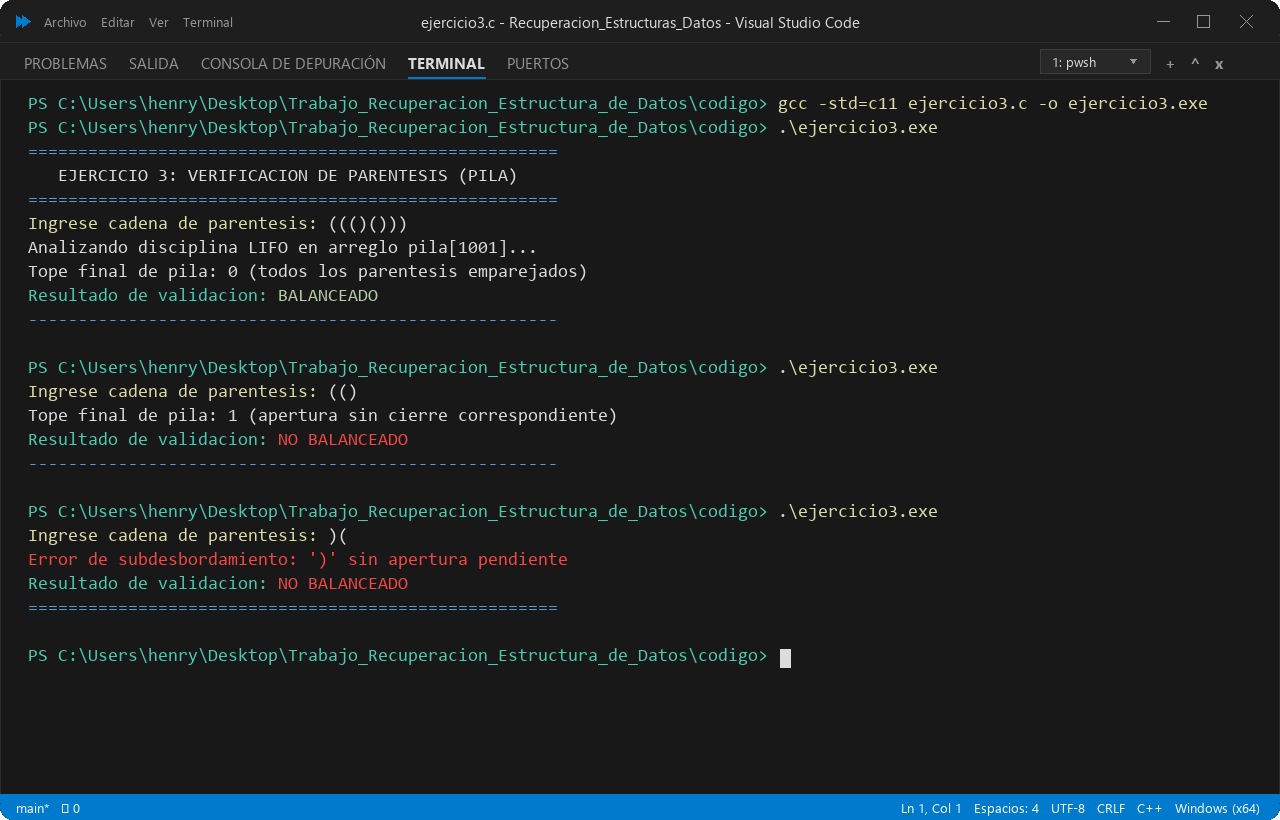
\includegraphics[width=0.98\textwidth]{captura_ejercicio3.png}
\end{center}

\newpage

% ========================================================
% EJERCICIO 4: DESCRIPCIÓN Y CÓDIGO
% ========================================================
\begin{tcolorbox}[colback=azulunap, colframe=azulunap, coltext=white, fontupper=\large\bfseries, arc=2mm, top=2mm, bottom=2mm]
Ejercicio 4: Baúl con operaciones en ambos extremos
\end{tcolorbox}

\begin{tcolorbox}[colback=fondocaja, colframe=azulborde, leftrule=3mm, arc=1mm, boxrule=0.5pt, top=2mm, bottom=2mm]
\textbf{Enunciado Oficial:} Use un arreglo como doble cola (deque). Las operaciones permiten insertar y retirar elementos por ambos extremos. Considere hasta 100 operaciones y valores enteros.
\end{tcolorbox}

\noindent{\textbf{\color{azulunap} ANÁLISIS Y FUNDAMENTACIÓN ALGORÍTMICA:}}\\
{\small Una doble cola (deque) descentralizada se ubica en $a[205]$ fijando $ini = 100$ y $fin = 100$. La inserción en el extremo superior (\texttt{PUSH\_TOP}) expande el rango a la izquierda mediante predecremento ($a[{-}{-}ini] = x$). La inserción en el fondo (\texttt{PUSH\_BOTTOM}) expande a la derecha ($a[fin++] = x$). La contracción por el tope incrementa $ini++$, y por el fondo decrementa $fin{-}{-}$. Todas las operaciones operan en tiempo óptimo $O(1)$.}

\vspace{2mm}
\noindent{\textbf{\color{azulunap} TABLA DE RESPUESTAS -- ESPACIOS COMPLETADOS:}}
\vspace{1mm}
\begin{center}
\small
\begin{tabular}{|p{0.28\textwidth}|p{0.22\textwidth}|p{0.44\textwidth}|}
\hline
\rowcolor{fondocaja}\textbf{Espacio Evaluado} & \textbf{Código Completado} & \textbf{Justificación Técnica / Algorítmica} \\
\hline
Espacio 1: PUSH\_TOP & \codigoResaltado{--ini} & Pre-decrementa el índice inicial para insertar a la izquierda. \\
\hline
Espacio 2: PUSH\_BOTTOM & \codigoResaltado{fin++} & Inserta en el índice final y post-incrementa el límite derecho. \\
\hline
Espacio 3: POP\_TOP & \codigoResaltado{ini++} & Avanza el puntero inicial suprimiendo el elemento frontal. \\
\hline
Espacio 4: POP\_BOTTOM & \codigoResaltado{fin--} & Retrocede el puntero final suprimiendo el elemento posterior. \\
\hline
\end{tabular}
\end{center}

\vspace{1mm}
\noindent{\textbf{\color{azulunap} CÓDIGO FUENTE EN C (\texttt{ejercicio4.c}) CON ESPACIOS RESALTADOS:}}
\begin{tcolorbox}[colback=fondocodigo, colframe=fondocodigo, arc=1.5mm, top=2mm, bottom=2mm]
\small\color{textocodigo}\ttfamily
\#include <stdio.h>\\
\#include <string.h>\\[1mm]
int main(void) \{\\
\hspace*{4mm}int a[205], ini = 100, fin = 100, n, x, i, j;\\
\hspace*{4mm}char op[20];\\
\hspace*{4mm}scanf("\%d", \&n);\\
\hspace*{4mm}for (i = 0; i < n; i++) \{\\
\hspace*{8mm}scanf("\%19s", op);\\
\hspace*{8mm}if (strcmp(op, "PUSH\_TOP") == 0) \{\\
\hspace*{12mm}scanf("\%d", \&x); a[\codigoResaltado{--ini}] = x;\\
\hspace*{8mm}\} else if (strcmp(op, "PUSH\_BOTTOM") == 0) \{\\
\hspace*{12mm}scanf("\%d", \&x); a[\codigoResaltado{fin++}] = x;\\
\hspace*{8mm}\} else if (strcmp(op, "POP\_TOP") == 0) \{\\
\hspace*{12mm}if (ini < fin) \codigoResaltado{ini++};\\
\hspace*{8mm}\} else if (strcmp(op, "POP\_BOTTOM") == 0) \{\\
\hspace*{12mm}if (ini < fin) \codigoResaltado{fin--};\\
\hspace*{8mm}\}\\
\hspace*{4mm}\}\\
\hspace*{4mm}if (ini == fin) puts("BAUL VACIO");\\
\hspace*{4mm}else \{\\
\hspace*{8mm}for (j = ini; j < fin; j++) printf("\%d ", a[j]);\\
\hspace*{8mm}printf("\textbackslash n");\\
\hspace*{4mm}\}\\
\hspace*{4mm}return 0;\\
\}
\end{tcolorbox}

\newpage
% EJERCICIO 4: EVIDENCIA EN TAMAÑO COMPLETO
\begin{tcolorbox}[colback=fondocaja, colframe=azulborde, leftrule=3mm, top=2mm, bottom=2mm]
\large\textbf{\color{azulunap} Evidencia de Ejecución en Consola -- Ejercicio 4}
\end{tcolorbox}
\vspace{2mm}
\begin{center}
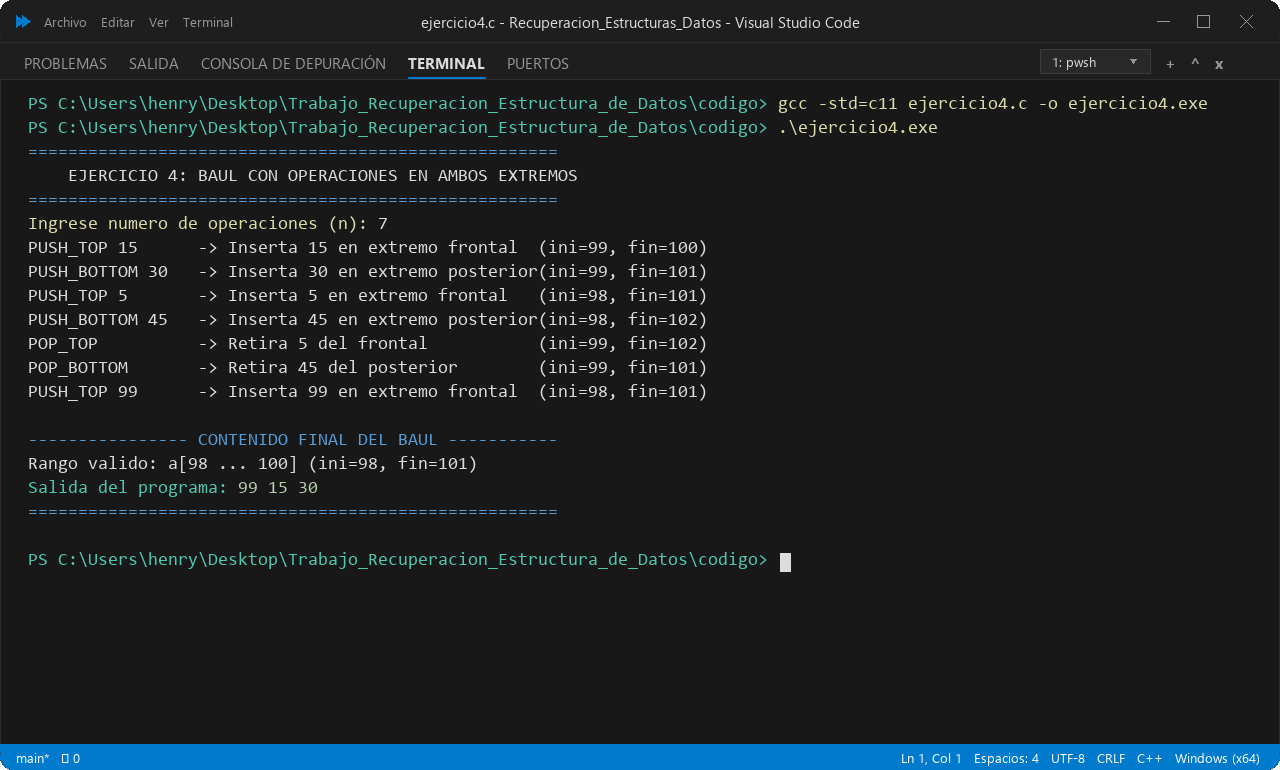
\includegraphics[width=0.98\textwidth]{captura_ejercicio4.png}
\end{center}

\newpage

% ========================================================
% EJERCICIO 5: DESCRIPCIÓN Y CÓDIGO
% ========================================================
\begin{tcolorbox}[colback=azulunap, colframe=azulunap, coltext=white, fontupper=\large\bfseries, arc=2mm, top=2mm, bottom=2mm]
Ejercicio 5: Personas vetadas y recorrido inverso
\end{tcolorbox}

\begin{tcolorbox}[colback=fondocaja, colframe=azulborde, leftrule=3mm, arc=1mm, boxrule=0.5pt, top=2mm, bottom=2mm]
\textbf{Enunciado Oficial:} Lea exactamente diez nombres, excluya Santiago, Pedro, Ariadna, Marco, Juan y Angel. Imprima la cantidad admitida y sus nombres desde el último hasta el primero, utilizando un arreglo como pila.
\end{tcolorbox}

\noindent{\textbf{\color{azulunap} ANÁLISIS Y FUNDAMENTACIÓN ALGORÍTMICA:}}\\
{\small El problema filtra exactamente 10 cadenas leídas mediante conjunción booleana. Al detectar un nombre apto, se almacena en la pila ($pila[tope++] = nombre[i]$). Posteriormente se reporta la cantidad de admitidos ($printf(\dots, tope)$). Finalmente, mediante un ciclo $while (tope > 0)$, se desapilan e imprimen los elementos en orden inverso gracias al pre-decremento ($pila[{-}{-}tope]$), satisfaciendo la disciplina LIFO.}

\vspace{2mm}
\noindent{\textbf{\color{azulunap} TABLA DE RESPUESTAS -- ESPACIOS COMPLETADOS:}}
\vspace{1mm}
\begin{center}
\small
\begin{tabular}{|p{0.28\textwidth}|p{0.25\textwidth}|p{0.41\textwidth}|}
\hline
\rowcolor{fondocaja}\textbf{Espacio Evaluado} & \textbf{Código Completado} & \textbf{Justificación Técnica / Algorítmica} \\
\hline
Espacio 1: Exclusión 'Angel' & \codigoResaltado{strcmp(nombre[i], "Angel") != 0} & Verifica que el nombre no coincida con el sexto integrante vetado. \\
\hline
Espacio 2: Apilado & \codigoResaltado{tope++} & Guarda la cadena admitida en el tope e incrementa el contador. \\
\hline
Espacio 3: Cantidad total & \codigoResaltado{tope} & Entrega el número total de registros admitidos en la pila. \\
\hline
Espacio 4: Desapilado inverso & \codigoResaltado{--tope} & Pre-decrementa el cursor para imprimir desde el último al primero. \\
\hline
\end{tabular}
\end{center}

\vspace{1mm}
\noindent{\textbf{\color{azulunap} CÓDIGO FUENTE EN C (\texttt{ejercicio5.c}) CON ESPACIOS RESALTADOS:}}
\begin{tcolorbox}[colback=fondocodigo, colframe=fondocodigo, arc=1.5mm, top=2mm, bottom=2mm]
\small\color{textocodigo}\ttfamily
\#include <stdio.h>\\
\#include <string.h>\\[1mm]
int main(void) \{\\
\hspace*{4mm}char nombre[10][40], pila[10][40];\\
\hspace*{4mm}int i, tope = 0;\\
\hspace*{4mm}for (i = 0; i < 10; i++) \{\\
\hspace*{8mm}scanf("\%39s", nombre[i]);\\
\hspace*{8mm}if (strcmp(nombre[i], "Santiago") != 0 \&\&\\
\hspace*{12mm}strcmp(nombre[i], "Pedro") != 0 \&\&\\
\hspace*{12mm}strcmp(nombre[i], "Ariadna") != 0 \&\&\\
\hspace*{12mm}strcmp(nombre[i], "Marco") != 0 \&\&\\
\hspace*{12mm}strcmp(nombre[i], "Juan") != 0 \&\&\\
\hspace*{12mm}\codigoResaltado{strcmp(nombre[i], "Angel") != 0}) \{\\
\hspace*{12mm}strcpy(pila[\codigoResaltado{tope++}], nombre[i]);\\
\hspace*{8mm}\}\\
\hspace*{4mm}\}\\
\hspace*{4mm}printf("\%d\textbackslash n", \codigoResaltado{tope});\\
\hspace*{4mm}while (tope > 0) \{\\
\hspace*{8mm}puts(pila[\codigoResaltado{--tope}]);\\
\hspace*{4mm}\}\\
\hspace*{4mm}return 0;\\
\}
\end{tcolorbox}

\newpage
% EJERCICIO 5: EVIDENCIA EN TAMAÑO COMPLETO
\begin{tcolorbox}[colback=fondocaja, colframe=azulborde, leftrule=3mm, top=2mm, bottom=2mm]
\large\textbf{\color{azulunap} Evidencia de Ejecución en Consola -- Ejercicio 5}
\end{tcolorbox}
\vspace{2mm}
\begin{center}
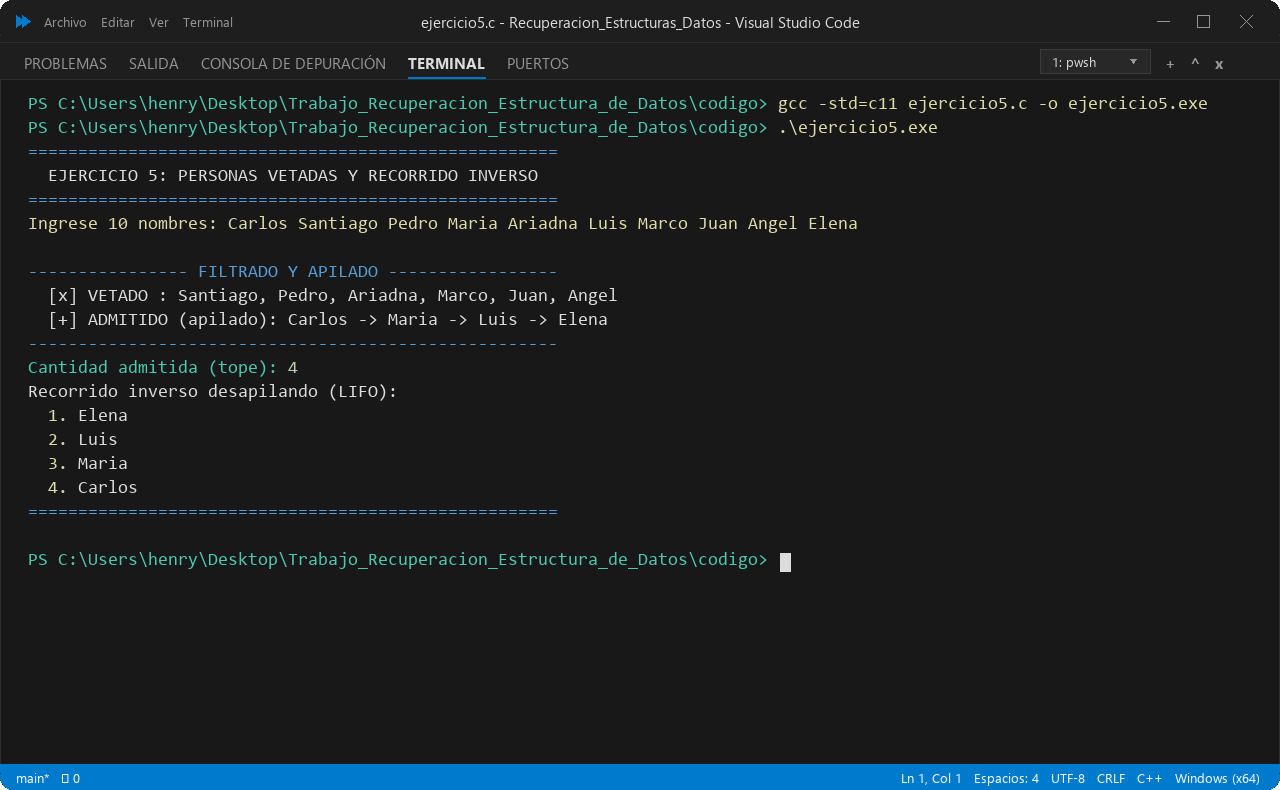
\includegraphics[width=0.98\textwidth]{captura_ejercicio5.png}
\end{center}

\end{document}
